\documentclass[a4paper]{article}
\usepackage[english]{babel}
\usepackage[utf8x]{inputenc}
% package for including graphics with figure-environment
\usepackage{graphicx}
\usepackage{hyperref}
% colors for hyperlinks
% colored borders (false) colored text (true)
\hypersetup{colorlinks=true,citecolor=black,filecolor=black,linkcolor=black,urlcolor=black}

% package for bibliography
\usepackage[authoryear,round]{natbib}
% package for header
\usepackage[automark]{scrlayer-scrpage}
\pagestyle{scrheadings}
\ihead[]{Bogdan Kyuchukov}
\ohead[]{\today}
\cfoot[]{\pagemark} 
\setheadsepline[122mm]{0.3mm}
\begin{document}
\title{
	\vspace{1cm}
	\Huge Verifying imperative programs \\ with Dafny \\
}

\vspace{1cm}

% if you are the only author, you might use the following
% \author{Name of student}	

% Insert here your name and correct mail address
\author{\Large \href{mailto:B.Kyuchukov@campus.lmu.de}{Bogdan Kyuchukov}
	\vspace{1cm}}

% name of the course and module
\date{
	\large Ludwig Maximilian University of Munich \\ Course: Deductive Software Verification \\
	\vspace{0.8cm}
	\large Lecturer: Prof. Gidon Ernst\\
	\vspace{1cm}
	\today
}

\maketitle
\setlength{\parindent}{0pt}

\vspace{2cm}
\begin{abstract}
	The goal of this work is to show how to formally reason
	about imperative programming constructs such as
	assignments, loops, arrays and especially about dynamically allocated objects. To be able to achieve that, basic
	Dafny constructs will be shown, such as functions, methods, pre- and postconditions. The discussion thereafter will move
	towards recursion and termination as well as inductive datatypes. Having learned from those chapters,
	loop invariants and their usage will be explored. Because analyzing objects in the heap is more challenging,
	searching and modifying arrays will be covered. The final chapter will include a detailed discussion about Dafny's
	dynamic frames and their significance.
\end{abstract}
\newpage
\tableofcontents
\newpage

\section{Introduction} % (fold)
\label{sec:introduction}
\subsection{Why Dafny?}
When software engineers encounter the field of formal methods and verification, this usually happens
in an academic setting, where proof techniques are learned and done by hand. Moreover, actually taking advantage
of those methods in practice involves a steep learning curve and lots of time. This unfortunately leads to less
acceptance of verification techniques in
an industry where fast time to market is essential \cite{reid2020makingformalmethodsnormal}. Dafny promises to solve those problems. As a programming
language designed to support specifications and proofs, it comes with an automated verifier that integrates
seamlessly into most modern IDEs \footnote{Integrated Development Environments (IDEs)} making rigorous verification part of the software development process,
thus reducing costly late-stage bugs that may be missed by testing.

\subsection{Dafny's build system}
The main idea in such verification-aware programming languages is that code is divided into two parts - the
specification part and the implementation part \cite{leino2023program}. The built-in verifier in Dafny acts as an
extended type checker and constantly proves that the provided implementation actually meets the behavior stated in
the specification part of the given function, method or class. This is done by transforming the code into an intermediary
that a tool called Boogie can understand. The correctness of the Boogie program implies the correctness of the
Dafny program. Boogie then generates first-order verification rules that are passed to the
Z3 SMT solver. Any violations of these conditions are passed back as verification errors \cite{Herbert2012}. This
process is visualized in Figure \ref{fig:build-system}.
\begin{figure}[h]
	\centering
	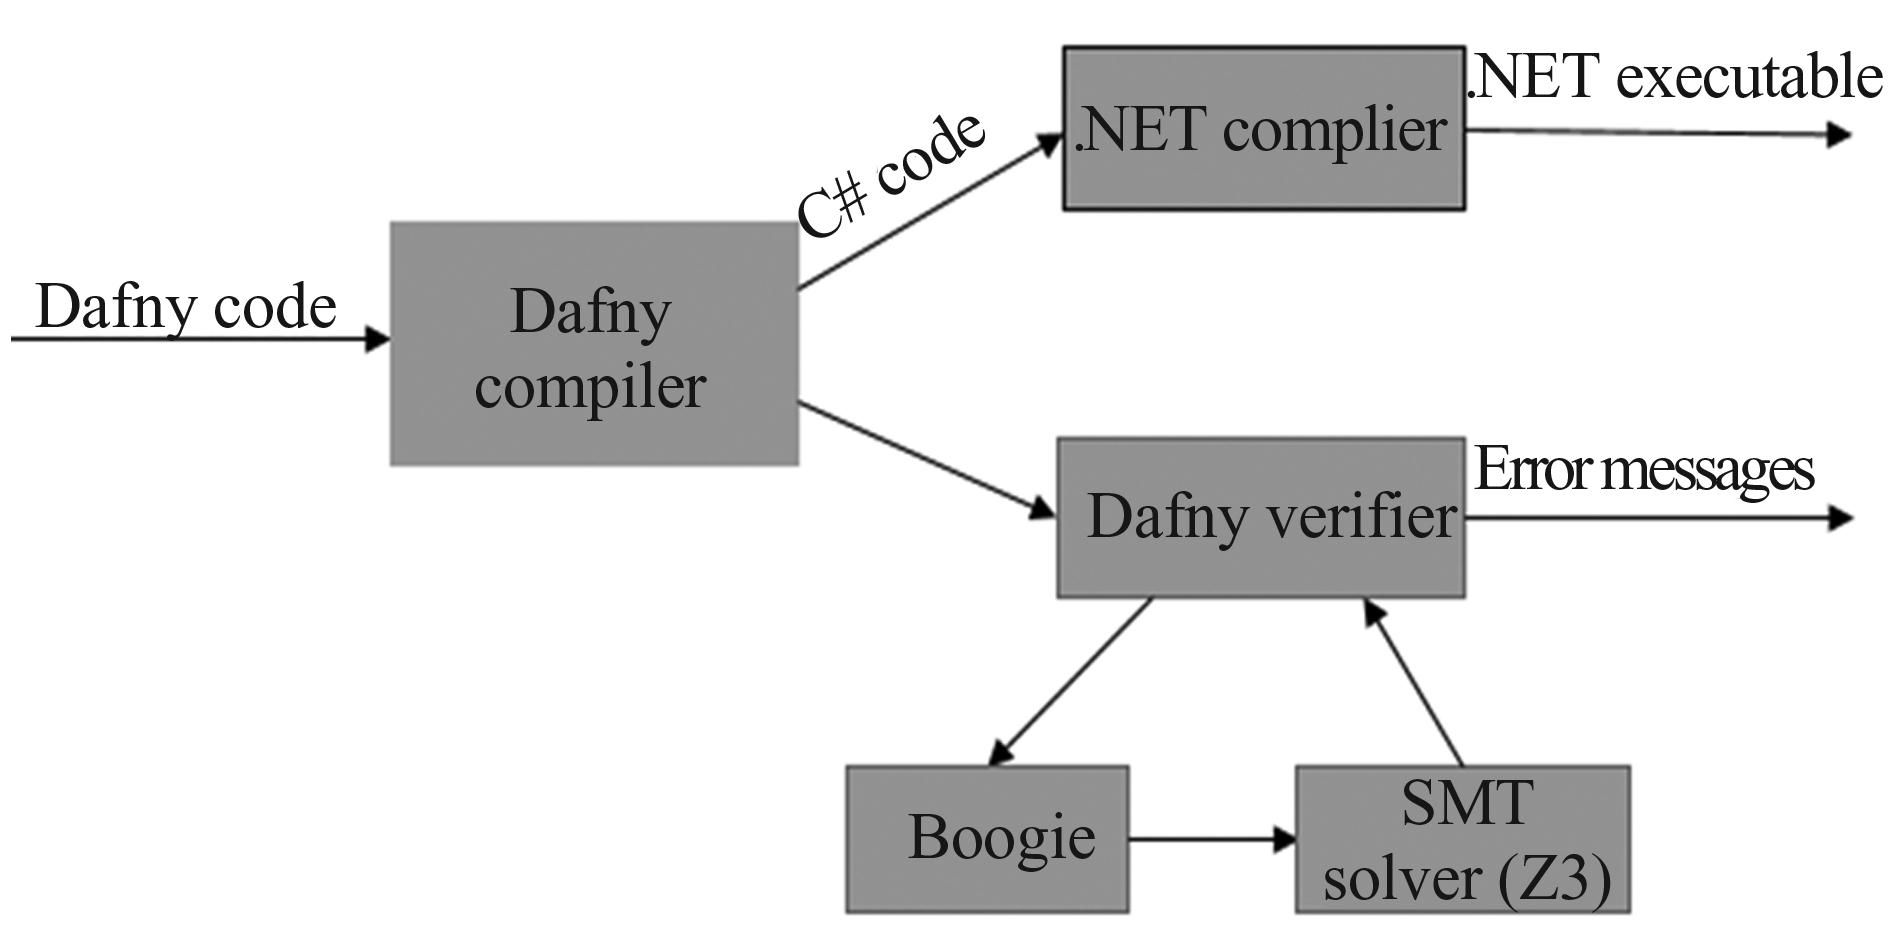
\includegraphics[width=0.7\textwidth]{images/dafny-infra.jpg}
	\caption{The Dafny build system as shown in \cite{Herbert2012}}
	\label{fig:build-system}
\end{figure}

%This work assumes the reader is familiarized with the fundamentals of program-semantics such as Floyd logic and
%Hoare triples, as they will be needed to explain Dafny more effectively. 
%weakest precondition $\mathcal{WP}$ and strongest postcondition $\mathcal{SP}$ of a program statement.
% Building blocks of Dafny
% Recursion and termination
% Inductive datatypes
% Searching & modifying arrays
% Dynamic Frames
\section{Building Blocks of Dafny} % (fold)
\label{sec:foundations}
Lorem ipsum dolor sit amet, consetetur sadipscing elitr, sed diam nonumy eirmod tempor invidunt ut labore
et dolore magna aliquyam erat, sed diam voluptua. At vero eos et accusam et justo duo dolores et ea rebum.
Stet clita kasd gubergren, no sea takimata sanctus est Lorem ipsum dolor sit amet. Lorem ipsum dolor sit amet,
consetetur sadipscing elitr, sed diam nonumy eirmod tempor invidunt ut labore et dolore magna aliquyam erat,
sed diam voluptua. At vero eos et accusam et justo duo dolores et ea rebum. Stet clita kasd gubergren,
no sea takimata sanctus est Lorem ipsum dolor sit amet.
\begin{verbatim}
	method Sequences() {
		var greetings := ["hey", "hola", "tjena"];
	  
		assert [1, 5, 12] + [22, 35] == [1, 5, 12, 22, 35];
	  
		var p := [1, 5, 12, 22, 35];
		assert p[2..4] == [12, 22];
		assert p[..2] == [1, 5];
		assert p[2..] == [12, 22, 35];
	  
		assert greetings[..1] == ["hey"];
		assert greetings[1..2] == ["hola"];
	}
\end{verbatim}


\section{Section about quotations} % (fold)
\label{sec:section_about_quotations}

In this section, an example for a literal quotation is given.

\begin{quotation}
	\emph{``A persona is a rich picture of an imaginary person who represents your core user group.''}
	\citep{Dix04}
\end{quotation}

Sometimes you might want to make use of the authors name within the text. Before, we used the command \texttt{citep\{\}}, which creates the brackets around author name and year. You can also use the \texttt{cite} command like this: \\

\cite{Dix04} defined the concept of persona as follows:
\begin{quotation}
	\emph{``A persona is a rich picture of an imaginary person who represents your core user group.''}
	\citep{Dix04}
\end{quotation}

You may notice, that this increases the readability of the text. \\

According to APA format\footnote{ American Psychological Association (APA)} there are some rules, when and how to include page numbers, when referring to literature.

\begin{quotation}
	\emph{``Include page numbers for any citations in the text of your paper that include direct quotations or refer to a specific part of the work you are referencing. Direct quotations must include a page number as part of the citation. The quoted material should be followed by a citation in parentheses that gives the author's name, the year in which the work was published, and the page number from which the quoted material appears.''}
	\citep{Hall}
\end{quotation}

Check out the example and recommendations of \cite{Hall} on \url{http://www.ehow.com/how_5689799_cite-numbers-apa-format.html}. In \LaTeX you can include the pages very easy. For example: \\

\citet[p. 86]{Baddeley:1974ts} stated:

\begin{quotation}
	\emph{``We hope that our preliminary attempts to begin answering the question will convince the reader, not necessarily that our views are correct, but that the question was and is well worth asking''}
	\citep[p. 86]{Baddeley:1974ts}
\end{quotation}

Note that in the first reference, we used \texttt{citet[]\{\}} in order to have brackets just around year and page number; later we used \texttt{citep[]\{\}}.

% section section_about_quotations (end)


\section{Section about references within the document} % (fold)
\label{sec:section_about_references_within_the_document}

If you want to refer to you own chapters, figures, tables or the like, you can make use of the \texttt{ref\{\}} command, for example:
\begin{itemize}
	\item section~\ref{sec:section_about_quotations} on page \pageref{sec:section_about_quotations}
\end{itemize}



% section section_about_references_within_the_document (end)

\subsection{Subsection within Foundations} % (fold)
\label{sub:subsection_within_foundations}
Lorem ipsum dolor sit amet, consetetur sadipscing elitr, sed diam nonumy eirmod tempor invidunt ut labore et dolore magna aliquyam erat, sed diam voluptua. At vero eos et accusam et justo duo dolores et ea rebum. Stet clita kasd gubergren, no sea takimata sanctus est Lorem ipsum dolor sit amet. Lorem ipsum dolor sit amet, consetetur sadipscing elitr, sed diam nonumy eirmod tempor invidunt ut labore et dolore magna aliquyam erat, sed diam voluptua. At vero eos et accusam et justo duo dolores et ea rebum. Stet clita kasd gubergren, no sea takimata sanctus est Lorem ipsum dolor sit amet.
% subsection subsection_within_foundations (end)

\subsection{Another subsection within Foundations} % (fold)
\label{sub:another_subsection_within_foundations}
Lorem ipsum dolor sit amet, consetetur sadipscing elitr, sed diam nonumy eirmod tempor invidunt ut labore et dolore magna aliquyam erat, sed diam voluptua. At vero eos et accusam et justo duo dolores et ea rebum. Stet clita kasd gubergren, no sea takimata sanctus est Lorem ipsum dolor sit amet. Lorem ipsum dolor sit amet, consetetur sadipscing elitr, sed diam nonumy eirmod tempor invidunt ut labore et dolore magna aliquyam erat, sed diam voluptua. At vero eos et accusam et justo duo dolores et ea rebum. Stet clita kasd gubergren, no sea takimata sanctus est Lorem ipsum dolor sit amet.
% subsection another_subsection_within_foundations (end)


% section foundations (end)

\section{Methodology} % (fold)
\label{sec:methodology}
Lorem ipsum dolor sit amet, consetetur sadipscing elitr, sed diam nonumy eirmod tempor invidunt ut labore et dolore magna aliquyam erat, sed diam voluptua \citep{Dix04}. At vero eos et accusam et justo duo dolores et ea rebum. Stet clita kasd gubergren, no sea takimata sanctus est Lorem ipsum dolor sit amet. Lorem ipsum dolor sit amet, consetetur sadipscing elitr, sed diam nonumy eirmod tempor invidunt ut labore et dolore magna aliquyam erat, sed diam voluptua. At vero eos et accusam et justo duo dolores et ea rebum. Stet clita kasd gubergren, no sea takimata sanctus est Lorem ipsum dolor sit amet.
% section methodology (end)

\section{Results} % (fold)
\label{sec:results}
Lorem ipsum dolor sit amet, consetetur sadipscing elitr, sed diam nonumy eirmod tempor invidunt ut labore et dolore magna aliquyam erat, sed diam voluptua \citep[p. 48]{Baddeley:1974ts}. At vero eos et accusam et justo duo dolores et ea rebum. Stet clita kasd gubergren, no sea takimata sanctus est Lorem ipsum dolor sit amet. Lorem ipsum dolor sit amet, consetetur sadipscing elitr, sed diam nonumy eirmod tempor invidunt ut labore et dolore magna aliquyam erat, sed diam voluptua. At vero eos et accusam et justo duo dolores et ea rebum. Stet clita kasd gubergren, no sea takimata sanctus est Lorem ipsum dolor sit amet.
% section results (end)

\section{Conclusion} % (fold)
\label{sec:conclusion}
Lorem ipsum dolor sit amet, consetetur sadipscing elitr, sed diam nonumy eirmod tempor invidunt ut labore et dolore magna aliquyam erat, sed diam voluptua. At vero eos et accusam et justo duo dolores et ea rebum. Stet clita kasd gubergren, no sea takimata sanctus est Lorem ipsum dolor sit amet. Lorem ipsum dolor sit amet, consetetur sadipscing elitr, sed diam nonumy eirmod tempor invidunt ut labore et dolore magna aliquyam erat, sed diam voluptua. At vero eos et accusam et justo duo dolores et ea rebum. Stet clita kasd gubergren, no sea takimata sanctus est Lorem ipsum dolor sit amet.
% section conclusion (end)


\newpage

\listoffigures
\bibliographystyle{apalike}
\bibliography{references}
\addcontentsline{toc}{section}{References}
\end{document}